% TODO L01 INTRODUCTION

\ifuniversity{recording}{\date{April 19, 2023}\setpicture[250]{apr21-o25a}\setcopyright{}}
\ifuniversity{ulm}{\date{April 18, 2023}\setpicture[250]{apr21-o25a}}
\ifuniversity{magdeburg}{\setpicture[70]{ovgu-autumn1}\setcopyright{Photo: Hannah Theile (OVGU)}}

\author{Thomas Thüm, Timo Kehrer, Elias Kuiter}
\lecture{Introduction}{introduction}

\inputuniversity{content/01-prelude}

\section{Introduction to Product Lines}
\subsection{Handcrafting and Customization}
\begin{frame}{What do these examples have in common?}
	\begin{mycolumns}[columns=3,widths={35,28},animation=none]
		\pic[width=\linewidth,trim=25 200 25 25,clip]{wedding}
		
		\pic[width=\linewidth]{shoes}
	\mynextcolumn
		\pic[width=\linewidth,trim=85 0 0 0]{eiffel-tower}
	\mynextcolumn
		\pic[width=\linewidth,trim=70 35 0 0]{draisine}
		
		~
		
		\uncover<2->{\begin{definition}{Customization \deutschertitel{Maßschneiderung}}
			\begin{itemize}
			\item aka.\ handcrafting
			\item labor-intensive production
			\item highly individual goods
			\end{itemize}
		\end{definition}}
	\end{mycolumns}
\end{frame}

\begin{frame}{Customization of Elevators}
	\begin{mycolumns}[columns=4,T]
		\centering\pic[width=\linewidth]{elevator1-out}

		two buttons
	\mynextcolumn
		\centering\pic[width=\linewidth]{elevator2-out2}

		one button
	\mynextcolumn
		\centering\pic[width=\linewidth]{elevator3-out}

		keyhole
	\mynextcolumn
		\centering\pic[width=\linewidth]{elevator2-out1}

		floor display
	\end{mycolumns}
\end{frame}

\begin{frame}{Customization of Elevators}
	\begin{mycolumns}[columns=4,widths={28,21,28,21},T]
		\centering\pic[width=\linewidth]{elevator1-in2}

		no button to close door
	\mynextcolumn
		\centering\pic[width=\linewidth]{elevator3-in1}

		two keyholes
	\mynextcolumn
		\centering\pic[width=\linewidth]{elevator4-in}

		keycard
	\mynextcolumn
		\centering\pic[width=\linewidth]{elevator2-in2}

		double tap for~undo
	\end{mycolumns}
\end{frame}

\subsection{Mass Production}
\begin{frame}[b]{\myframetitle}
	\vspace{-\textheightoftitle}
	\begin{mycolumns}[b]
		\begin{definition}{Mass Production \deutschertitel{Massenproduktion}\mysource{\fospl\mypages{3--4}}}
			\begin{itemize}
			\item consequence of industrialization
			\item goods are produced from standardized parts
			\item improved productivity wrt.\ handcrafting
			\item reduced costs, improved quality
			\item but: (almost) no individualism
			\end{itemize}
		\end{definition}
		\uncover<2->{\begin{example}{Principle: One Size Fits All}
			\begin{itemize}
			\item t-shirts: XS, S, M, L, XL, XXL
			\item swiss-army knife \deutsch{Eierlegende Wollmilchsau}
			\end{itemize}
		\end{example}
		\centering\pic[width=.45\linewidth]{wollmilchsau}}
	\mynextcolumn
		\pic[width=\linewidth]{swiss-army-knife}
		\uncover<3->{\begin{note}{Mass Production for Software?\mysource{\fospl\mypage{7}}}
			\mycite{The idea is to provide software that satisfies the needs of most customers, which leads almost automatically to the situation, in which customers miss desired functionality and are overwhelmed with functionality they do not need actually (just think of any contemporary office or graphics program). It is often this generality that makes software complex, slow, and buggy.}
		\end{note}}
	\end{mycolumns}
\end{frame}
% industrial revolution/era:
% - John Hall, exchangable parts 1826, 25 years of trials (source?)
% - Henry Ford/Ransom Olds, production/assembly line, 1901 (source?)
% - 1961 first industrial roboter at General Motors
% - 1980s automatic assembly lines

\subsection{Mass Customization}
\begin{frame}{About Every Second Car is Unique}
	\centering\pic[width=.66\linewidth]{many-cars}
\end{frame}
\begin{frame}{\myframetitle\ \deutschertitel{Kundenindividuelle Massenproduktion}}
	\begin{mycolumns}[widths={45}]
		\begin{definition}{Mass Customization\mysource{\fospl\mypage{4}}}
			\begin{itemize}
			\item = mass production + customization
			\item customized, individual goods at costs similar to mass production
			\end{itemize}
		\end{definition}
		\myexampletight{Car Configuration}{\pic[width=\linewidth]{toyota-aygo-wheels}}
	\mynextcolumn
		\myexampletight{Car Production}{\pic[width=\linewidth,trim=0 50 0 240,clip]{car-manufacturing}}
		\begin{example}{Other Domains}
			bikes, computers, electronics, tools, medicine, clothing, food, financial services, \ldots, software?
		\end{example}
	\end{mycolumns}
\end{frame}

\begin{frame}{Mass Customization for Software?}
	\begin{mycolumns}[b,widths={55},animation=none]
		\begin{definition}{Mass Customization for Software?}
			\begin{itemize}
			\item customization: individual software developed using Waterfall model or Scrum
			\item mass production: standard software developed once for millions or billions of users (e.g.,~Whatsapp messenger)
			\item mass customization: software product lines
			\end{itemize}
		\end{definition}
		\uncover<2->{\begin{note}{Why Software Product Lines?}
			\begin{itemize}
			\item resource limitations: memory, performance, energy
			\item different hardware
			\item different laws
			\item goal: avoid expensive customization
			\item how is software developed?
			\end{itemize}
		\end{note}}
	\mynextcolumn
		\pic[width=\linewidth,trim=250 0 0 0,clip]{car-tower}
	\end{mycolumns}
\end{frame}

\subsection{Recap: The Software Life Cycle}
\begin{frame}{The Project Cartoon}
	\renewcommand{\projectcartoonwidth}{.135}
	\uncover<2-|handout:1-2>{\alt<-8|handout:1>{\hprojectcartoon{01}{how the customer explained it}}{\alt<9|handout:2>{\hprojectcartoon{01}{Requirements}}{\projectcartoon{01}{Requirements}}}}% requirements
	\uncover<3->{\alt<-8,10-|handout:1>{\hprojectcartoon{02}{how the project leader understood it}}{\projectcartoon{02}{how the project leader understood it}}}% modeling
	\uncover<4->{\alt<-8,10-|handout:1>{\hprojectcartoon{03}{how the analyst designed it}}{\projectcartoon{03}{how the analyst designed it}}}% architecture and design
	\uncover<5->{\alt<-8,10-|handout:1>{\hprojectcartoon{04}{how the programmer implemented it}}{\projectcartoon{04}{how the programmer implemented it}}}% implementation
	\uncover<6->{\alt<-8,10-|handout:1>{\hprojectcartoon{05}{what the beta testers received}}{\projectcartoon{05}{what the beta testers received}}}% testing
	\uncover<7->{\alt<-8,10-|handout:1>{\hprojectcartoon{10}{how it was supported}}{\projectcartoon{10}{how it was supported}}}% maintenance
	\uncover<8->{\alt<-8|handout:1>{\hprojectcartoon{13}{what the customer really needed}}{\alt<9>{\hprojectcartoon{13}{Product}}{\projectcartoon{13}{Product}}}}% customer / SE II
	\\
\end{frame}

\begin{frame}{\myframetitle\ \deutschertitel{Software-Lebenszyklus}}
	\waterfallcartoon\\
\end{frame}

\subsection{Features and Products of a Domain}
\begin{frame}{What is a Feature?}
	\begin{mycolumns}[widths={45},t]
		\uncover<2->{\begin{definition}{Feature \deutsch{Feature} \mysource{\fospl\mypage{18}}}
			\mycite{A \emph{feature} is a characteristic or end-user-visible behavior of a software system.}
		\end{definition}}
		\centering\xkcd{2369}{width=.9\linewidth,trim=35 35 35 35,clip}
	\mynextcolumn
		\uncover<3->{\begin{note}{Feature in a Product Line \mysource{\fospl\mypage{18}}}
			\mycitebegin Features are used in product-line engineering
			\begin{itemize}
				\item to specify and communicate commonalities and differences of the products between stakeholders \deutsch{Akteure} and
				\item to guide structure, reuse, and variation across all phases of the software life cycle.\myciteend
			\end{itemize}
		\end{note}}
		\renewcommand{\projectcartoonwidth}{.18}\scriptsize
		\uncover<4->{\waterfallcartoon}\\
	\end{mycolumns}
\end{frame}
% TODO picture of a program highlighting one or two features? settings? changelog? marketing description of new features (Github?)?

% goals of features
%a distinctively identifiable functional abstraction that must be implemented, tested, delivered, and maintained” (Kang et al.
%a product characteristic from user or customer views, which essentially consists of a cohesive set of individual requirements” (Chen et al.
%an optional or incremental unit of Zave 2003) 

\begin{frame}{What is a Product?}
	\begin{mycolumns}[t,animation=none]
		\begin{definition}{Product \deutsch{Produkt} \mysource{\fospl\mypage{19}}}
			\mycite{A \emph{product of a product line} is specified by a valid feature selection (a subset of the features of the product line). A feature selection is \emph{valid} if and only if it fulfills all feature dependencies.}
		\end{definition}
		\uncover<2->{\begin{note}{Note on Terminology}
			\begin{itemize}
				\item in this course:\\product = product variant = variant
				\item software product: a product consisting only of software
				\item software is more than a program: requirements, models, source code, tests, documentation
				\item this course focuses on source code
			\end{itemize}
		\end{note}}
		% TODO exemplify difference between hardware product, software product (VLC?), and program (reuse pictures from before)
	\mynextcolumn
		\uncover<3->{\myexampletight{Product Map for Eclipse (excerpt)}{
			\pic[width=\linewidth,trim=0 460 635 0,clip]{eclipse-product-map}
		}}
	\end{mycolumns}
\end{frame}
% TODO Venn diagram could also be a good visualization: products correspond to sets and features to set elements

\begin{frame}{What is a Domain?}
	\begin{mycolumns}[animation=none]
		\begin{definition}{Domain \deutsch{Domäne} \mysource{\fospl\mypage{19}}} % TODO cite CE00 here too?
			\mycitebegin A \emph{domain} is an area of knowledge that:
			\begin{itemize}
				\item is scoped to maximize the satisfaction of the requirements of its stakeholders,
				\item includes a set of concepts and terminology understood by practitioners in that area,
				\item and includes the knowledge of how to build software systems (or parts of
				software systems) in that area.\myciteend
			\end{itemize}
		\end{definition}
		\uncover<2->{\begin{note}{Features of a Domain}
			\begin{itemize}
				\item a feature is a domain abstraction
				\item identification of features in a domain requires domain expertise
				\item later: select features for a product line?
			\end{itemize}
		\end{note}}
	\mynextcolumn
		\pic[width=.5\linewidth]{many-cars}

		\hfill\xkcd{2369}{width=.5\linewidth,trim=35 35 35 35,clip}\hfill{}

		\hfill\pic[width=.5\linewidth]{eclipse-luna}
	\end{mycolumns}
\end{frame}
% TODO add more examples for domains

\subsection{Software Product Line}
\begin{frame}{\myframetitle}
	\begin{mycolumns}[widths={78},columns=1]
		\begin{definition}{Software Product Line \mysource{\seiwhitepaperspl\mypage{5}}}
			\mycitebegin A \emph{software product line} is
			\begin{itemize}
				\item a set of software-intensive systems \uncover<2->{\myexampletight{}{aka.\ products or variants}}
				\item that share a common, managed set of features \uncover<3->{\myexampletight{}{common set, but not all products have all features in common}}
				\item satisfying the specific needs of a particular market segment or mission \uncover<4->{\myexampletight{}{aka.\ domain \deutsch{Domäne, Einsatzgebiet, Marktsegment}}}
				\item and that are developed from a common set of core assets in a prescribed way.\myciteend \uncover<5->{\myexampletight{}{aka.\ planned, structured reuse \deutsch{Wiederverwendung von vorbereiteten Teilen}}}
				\mysource{\href{https://resources.sei.cmu.edu/library/asset-view.cfm?assetID=513819}{Software Engineering Institute, Carnegie Mellon University}}
			\end{itemize}
		\end{definition}
	\end{mycolumns}
\end{frame}
% variants / platforms / domain / variant generation
% configurable software, highly-configurable software, variable software, software variation

\subsection{Product-Line Engineering}
\begin{frame}{\myframetitle}
	\begin{mycolumns}[animation=none]
		\begin{definition}{Product-Line Engineering\mysource{\sple\mypage{14}}}
			\mycite{\emph{Software product-line engineering} is a paradigm to develop software applications (software-intensive systems and software products) using software platforms and mass customization.}
%			\begin{itemize}
%			\item aka.\ product-line development \mysource{\seiwhitepaperspl\mypage{207}}
%			\end{itemize}
		\end{definition}
		\uncover<2->{\begin{note}{Promises of Product Lines \mysource{\fospl\mypages{9--10}}}
			\begin{itemize}
				\item tailor-made \deutsch{Maßschneiderung}
				\item reduced costs \deutsch{Kostenreduzierung}
				\item improved quality \deutsch{Qualitätssteigerung}
				\item reduced time-to-market \deutsch{Reduzierung der Produktentwicklungszeit}
			\end{itemize}
		\end{note}}
	\mynextcolumn
		\vspace{-5mm}
		\uncover<3->{\mynotetight{Idea of Product-Line Engineering}{
			Reduce effort per product by means of an up-front investment for the product line:
			
			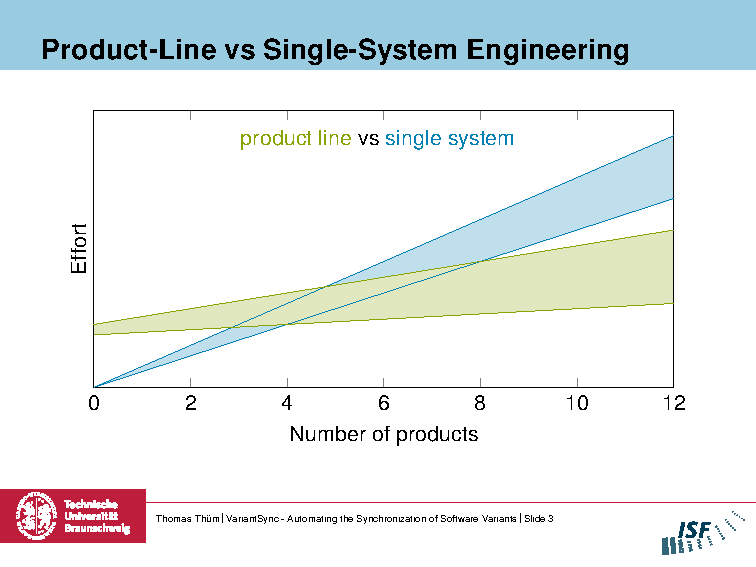
\includegraphics[width=\linewidth,trim=30 60 30 50,clip]{product-line-vs-single-system}
		}}
		\uncover<4->{\begin{definition}{Single-System Engineering}
			\begin{itemize}
			%\item aka.\ single-system development \mysource{\seiwhitepaperspl\mypage{7}}
			\item \deutsch{Einzelsystementwicklung}
			\item classical software development that is not considered as product-line engineering
			\end{itemize}
		\end{definition}}
	\end{mycolumns}
\end{frame}

% product-line hall of fame
% success stories: Boing, Bosch, Hewlett Packard, Toshiba, General Motors \mysource{\fospl}

% TODO \subsection{Running Examples?}
% \fospl: data management for embedded systems, product line of a graph library

% not software, not running: financial services (or in \lecturemodeling?), bikes, shoes, notebooks, ...
% Linux, Graph Product Line \lectureruntime\ or \lecturecloneandown, Configurable Database, Elevator Product Line, Printer product lines, Car configurators, software ecosystem (Browser plug-ins, IDE plug-ins)

% elevators: pictures from various elevators (OVGU, UULM, Bern), invisible end-user-visible features (e.g., double click for deselection)
% if you do this at home: do not select all stops before you know it is working

% how many examples in first lecture? move certain examples in later lectures? if so, which ones?
%\subsection{Automotive Systems}
% car configurators
% history? number of variants over time?
%\subsection{Notebooks}
% lenovo, microsoft, apple
%\subsection{Printer (Firmware)}
% real printers, 3d printers
% 30 printers per year, more examples
% XKCD: all-in-one paper processor
%\subsection{Operating Systems}
% windows, linux!!!, android
% Linux: where is it used? on which principal hardware? how many instances are running world wide? how many commits and developers? how many versions have been release and since when? screenshot how it looks like when linux is configured
% apps?
%\subsection{Integrated Development Environments}
% eclipse
%\subsection{Browsers}
% plug-ins

% apps! in market store android, iOS
% ecos, packages in debian

%\subsection{Beyond Software}
% financial products by KfW, bikes, shoes, muesli, Subway, headphones, lego, detergents, furniture (handcrafted vs standardized vs product line), kitchens
% brompton: picture in ulm slides

% zoo of animals/tools

% historical development? exchangable parts, production lines, automated product lines, ...
% all-in-one solution vs custom development? software for German fire departments
% all-in-one application software vs embedded software
% reasons for custom development: 

% goal of the lecture

%\subsection{Features}

%\subsection{Software Product Lines}
%% product-line engineering
%\begin{frame}{Who Produces Only One Product?}
%	\href{https://pxhere.com/en/photo/920906}{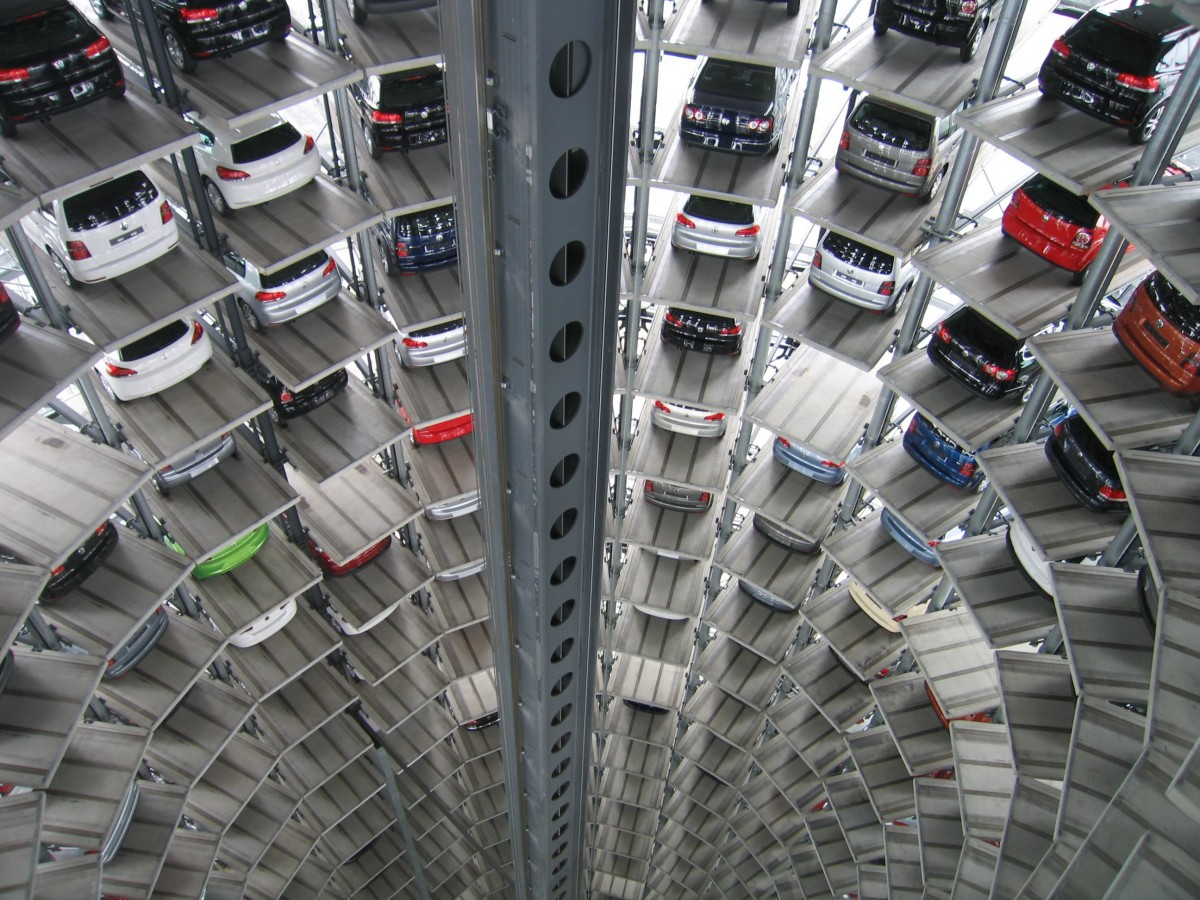
\includegraphics[width=.6\linewidth]{car-tower}}
%\end{frame}

%\subsection{Single System}
%% single-system engineering
%
%\begin{frame}{Greenfield Development? \deutschertitel{Auf der grünen Wiese?}}
%	\href{https://github.com/SoftVarE-Group/SlideTemplate/blob/main/pics/nature/may21-ulm.jpg}{\includegraphics[width=.6\linewidth]{may21-ulm}}
%\end{frame}



% add illustration for variants/versions (space/time) by icons of word/excel/powerpoint/one note/... over the years




% Apel 2013, Page 49
%Compile-time variability is decided before or at compile time.
%Load-time variability is decided after compilation when the program is started.
%With run-time variability, decisions can be made and changed during program
%execution.



% explain configurators vs selectors? for example, iPhone is available is produced in any combination and then selled, still there are selectors to find the right product easily. cf. ebay/amazon




% history on product lines? how old are product lines and ideas discussed in this lecture?





\lessonslearned{
	\item mass customization\\= mass production + customization
	\item features, products, domains
	\item software product lines
	\item product-line engineering
}{
	\item \fospl\mychapter{1}\mypages{3--15} --- introduction close to this lecture, further examples
	\item \seiwhitepaperspl\mypages{2--8} --- what is not a product line?
	% TODO add further reference? \sple\mypage{14}
}{
	\begin{itemize}
		\item What other examples of product lines do you know?
		\item Exemplify the differences between feature, product, domain, and product line for these examples.
		\item Are these product lines related to software?
	\end{itemize}
}

\section{Challenges of Product Lines}
\subsection{Software Clones}
\begin{frame}{\myframetitle}
	\frameSoftwareClones
\end{frame}

\subsection{Feature Traceability}
\begin{frame}{\myframetitle}
	\begin{mycolumns}[widths={40}]
		%\mydefinition{Feature Traceability \mysource{\fospl\mypage{54}}}{\mycite{Feature traceability is the ability to trace a feature from the problem space (for example, the feature model) to the solution space (that is, its manifestation in design and code artifacts).}}
		\begin{definition}{Feature Traceability}
			Feature traceability is the ability to trace a feature throughout the software life cycle (i.e., from requirements to source code).
		\end{definition}
		\begin{example}{Intuition on Feature Traceability}
			find feature 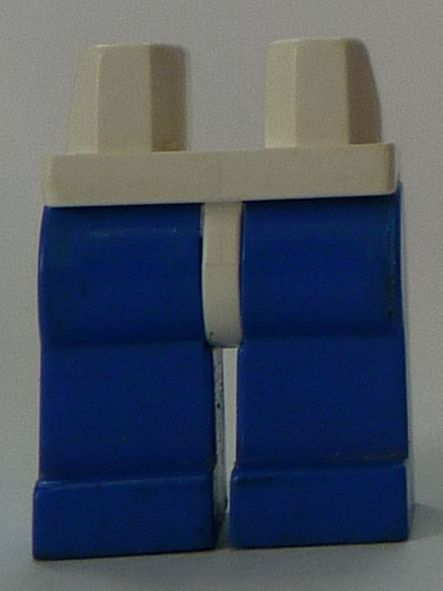
\includegraphics[width=.17\linewidth]{pants-blue} in product 
\includegraphics[width=.17\linewidth]{230}
		\end{example}
	\mynextcolumn
		\myexampletight{Feature Traceability with Colored Source Code}{\picDark[width=\linewidth]{feature-traceability}}
	\end{mycolumns}
\end{frame}

\subsection{Automated Generation}
\begin{frame}{\myframetitle}
	\begin{mycolumns}[columns=3,widths={37,7},animation=none]
		\myexampletight{Features}{
			\foreach \animation/\handout/\page in {1-2/0/5,3-4/0/6,5-6/0/7,7-8/0/8,9-10/0/9,11-/1/10} {%
				\only<\animation|handout:\handout>{
\includegraphics[width=\linewidth,page=\page,trim=45 0 45 0,clip]{lego}}%
			}%
		}
	\mynextcolumn
		\centering\Huge$\Rightarrow$
	\mynextcolumn
		\myexampletight{Products}{
			\foreach \animation/\handout/\page in {1/0/3,2-3/0/11,4-5/0/12,6-7/0/13,8-9/0/14,10-11/0/15,12-/1/18} {%
				\only<\animation|handout:\handout>{
\includegraphics[width=\linewidth,page=\page]{lego}}%
			}%
		}
	\end{mycolumns}
\end{frame}
\begin{frame}{\myframetitle}
	\begin{mycolumns}[widths={45},animation=none]
		\begin{example}{Product Line with Features}
			\only<1-2|handout:0>{
\includegraphics[width=\linewidth]{metaproduct}}%
			\only<3->{
\includegraphics[width=\linewidth]{metaproduct2}}%
		\end{example}
	\mynextcolumn
		\begin{definition}{Goal}
			\begin{itemize}
			\item automatic generation of products
			\item based on a (descriptive) selection of features
			\end{itemize}
		\end{definition}
		\uncover<2->{\begin{note}{Challenges}
			\begin{itemize}
			\item how to map features to source code?
			\item how to combine source code of multiple features?
			\item how to define valid combinations of features?
			\end{itemize}
		\end{note}}
	\end{mycolumns}
\end{frame}

\subsection{Combinatorial Explosion}
\begin{frame}{\myframetitle}
	\begin{mycolumns}[widths={49}]
		\myexampletight{Combinatorial Explosion}{
			\includegraphics[width=\linewidth,page=6]{cit-plots}%
			\small%
			\begin{itemize}
				\item assumption: all combinations of features are valid
				\item 33 features: a unique combination for every human
				\item 320 features: more combinations than atoms in the universe
			\end{itemize}
		}
	\mynextcolumn
		\myexampletight{Industrial Configuration Spaces \mysource{\evaluatingsharpsatsolvers}}{
			\evaluatingsharpsatsolverslink{\includegraphics[width=\linewidth,page=6,trim=50 210 320 440,clip]{2020/2020-VaMoS-Sundermann}}%
			\small%
			\begin{itemize}
				\item in practice: not all combinations of features valid
				\item many industrial product lines too large to specify all valid combinations separately
				\item largest automotive product line has about $1.7 \cdot 10^{1534}$ products
			\end{itemize}
		}
	\end{mycolumns}
\end{frame}
\begin{frame}{\myframetitle}
	\centering\href{https://github.com/SoftVarE-Group/Slides/blob/main/2021/2021-02-10-VaMoS-SharpSATApplications.pdf}{\includegraphics[height=\textheightwithtitle,page=9,trim=60 15 15 5,clip]{2021/2021-02-10-VaMoS-SharpSATApplications}}
\end{frame}

\subsection{Feature Interactions}
\begin{frame}{\myframetitle}
	\begin{mycolumns}
		\only<1-2|handout:0>{
\includegraphics[width=\linewidth,page=24]{lego}}%
		\only<3->{
\includegraphics[width=\linewidth,page=25]{lego}}%
	\mynextcolumn
		\begin{example}{Example Interaction}
			phone 
\includegraphics[width=.14\linewidth]{phone} cannot be used with helmet 
\includegraphics[width=.14\linewidth]{helmet}
		\end{example}
		\uncover<2->{\begin{note}{Challenges}
			\begin{itemize}
			\item interaction typically unknown in advance
			\item interactions occur in some but not all combinations
			\item challenge for quality assurance
			\end{itemize}
		\end{note}}
	\end{mycolumns}
\end{frame}
\begin{frame}{\myframetitle}
	\begin{mycolumns}[columns=3,widths={13,74},animation=none]
	\mynextcolumn
		\myexampletight{Invalid Car Configurations}{\picDark[width=\linewidth]{bmw-series1-confassistant-bluetooth}}
	\mynextcolumn
	\end{mycolumns}
\end{frame}

\subsection{Continuing Change and Growth}
\begin{frame}{\myframetitle}
	\begin{mycolumns}[widths={42}]
		\begin{definition}{Lehman's Laws of Software Evolution (excerpt) \mysource{\lehmanslaws}}
			\begin{itemize}
				\item Continuing Change: systems must be continually adapted to stay satisfactory % E-type systems must be continually adapted else they become progressively less satisfactorv.
				\item Increasing Complexity: complexity increases during evolution unless work is done to maintain or reduce it % As an E-type system evolves its complexity increases unless work is done to maintain or reduce it.
				%\item Self Regulation: %E-type system evolution process is self regulating with distribution of product and process measures close to normal.
				%\item Conservation of Organizational Stability (invariant work rate): %The average effective global activity rate in an evolving E-type system is invariant over product lifetime.
				%\item Conservation of Familiarity: satisfactory evolution excludes excessive growth %As an E-type system evolves all associated with it, developers, sales personnel, users, for example, must maintain mastery of its content and behaviour to achieve satisfactory evolution. Excessive growth diminishes that mastery. Hence the average incremental growth remains invariant as the system evolves.
				\item Continuing Growth: functionality must be continually increased to maintain user satisfaction %The functional content of E-type systems must be continually increased to maintain user satisfaction over their lifetime.
				\item Declining Quality: quality will decline unless rigorously maintained and adapted to operational environment changes %The quality of E-type systems will appear to be declining unless they are rigorously maintained and adapted to operational environment changes.
				%\item Feedback System: %E-type evolution processes constitute multi-level, multi-loop, multi-agent feedback systems and must be treated as such to achieve significant improvement over any reasonable base.
			\end{itemize}
		\end{definition}
	\mynextcolumn
		\begin{note}{Essence of the Laws}
			\begin{itemize}
				\item software that is used will be modified
				\item when modified, its complexity will increase (unless one does actively work against it)
			\end{itemize}
		\end{note}
		\begin{example}{Consequences for Product Lines}
			\begin{itemize}
				\item number of features and size of implementation increases over time
				\item discussed challenges increase over time
					\begin{itemize}
						\item more software clones
						\item harder to trace features
						\item automated generation more urgent
						\item increasing combinatorial explosion
						\item more feature interactions
					\end{itemize}
			\end{itemize}
		\end{example}
	\end{mycolumns}
\end{frame}

\begin{frame}{Evolution of the Linux Kernel}
	\begin{mycolumns}
		\begin{example}{}
			\begin{itemize}
				\item about $60,000$ commits per year
				\item in peak weeks: new commit every 5 minutes
				\item in average weeks: every 9 minutes
			\end{itemize}
		\end{example}
	\mynextcolumn
		\vspace{-\textheightoftitle}
		\picDark[width=\linewidth,trim=100 70 110 80,clip]{linux-stack-plot}
	\end{mycolumns}
	\twodimensionalanalysislink{\includegraphics[width=.8\linewidth,page=1,trim=80 420 80 260,clip]{2019/2019-VariVolution-Thuem}}
\end{frame}

\begin{frame}{Evolution of the Linux Kernel}
	\begin{mycolumns}
		\myexampletight{Size of the Code Base}{
			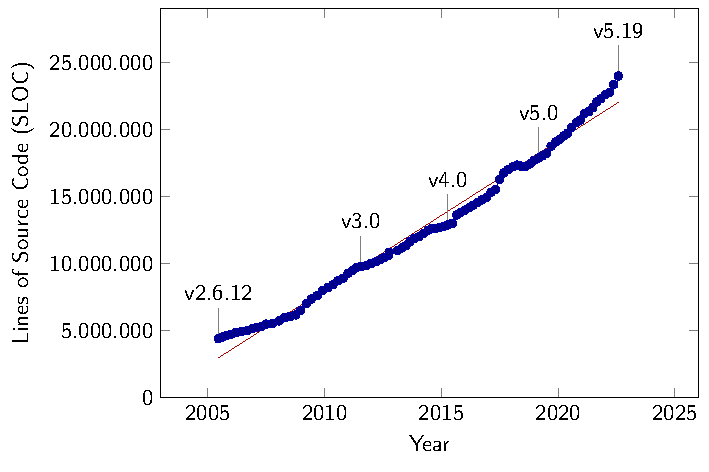
\includegraphics[width=\linewidth,page=1]{linux-plots}%
			\begin{itemize}
				\item from 4 to 24 millions in 17 years
				\item about one million LOC added every year
				\item about 3,000 LOC per day
			\end{itemize}
		}
	\mynextcolumn
		\myexampletight{Number of Features}{
			\includegraphics[width=\linewidth,page=2]{linux-plots}%
			\begin{itemize}
				\item about 800 new features every year
				\item about 15 new features every week
				\item in 2018 four times more features than in 2005
			\end{itemize}
		}
	\end{mycolumns}
\end{frame}

\begin{frame}{Evolution of the Linux Kernel}
	\begin{mycolumns}
		\myexampletight{Number of Products}{
			\includegraphics[width=\linewidth,page=3]{linux-plots}%
			\begin{itemize}
				\item number of products grows by factor 100.000 each month
				\item the current kernel is likely to have more than $10^{1500}$ products
			\end{itemize}
		}
	\mynextcolumn
		\myexampletight{Time to Count Products}{
			\includegraphics[width=\linewidth,page=4]{linux-plots}%
			\begin{itemize}
				\item most kernel versions before 2006 can be computed within 1 minute
				\item most kernel versions after 2006 cannot be computed within 1 hour
			\end{itemize}
		}
	\end{mycolumns}
\end{frame}

% costs: development, investment, maintenance, logistic, production
% customer needs?


\lessonslearned{
	\item why are product lines challenging?
	\item selected challenges:
		\begin{enumerate}
		\item software clones
		\item feature traceability
		\item automated generation
		\item combinatorial explosion
		\item feature interactions
		\item continuous growth
		\end{enumerate}
}{
	\item[] see later lectures
}{
	\begin{itemize}
		\item Form groups of 2--3 students
		\item Explain 2--3 of the six challenges to your colleagues
		\item Can you find own examples for these challenges?
	\end{itemize}
}

\section{Course Organization}
\subsection{What You Should Know}

\begin{frame}{\myframetitle{}}
	\begin{mycolumns}
		\mynote{Fundamentals of Software Engineering}{
			\begin{itemize}
				\item development processes
				\item object-oriented programming
				\item design patterns
				\item UML class diagrams
				\item modularity
			\end{itemize}
			\ifuniversity{magdeburg}{$\Rightarrow$ \emph{Software Engineering}}
		}
	\mynextcolumn
		\mynote{Fundamentals of Theoretical Computer Science}{
			\begin{itemize}
				\item set theory
				\item propositional logic
				\item complexity theory
			\end{itemize}
			\ifuniversity{magdeburg}{
				$\Rightarrow$ \emph{Logik}\\
				$\Rightarrow$ \emph{Grundlagen der Theoretischen Informatik I}
			}
		}

		\mynote{Exercise}{
			solid programming skills in Java

			\ifuniversity{magdeburg}{
				$\Rightarrow$ \emph{Einführung in die Informatik}\\
				$\Rightarrow$ \emph{Algorithmen und Datenstrukturen}
			}
		}
	\end{mycolumns}
\end{frame}

\subsection{What You Will Learn}

\begin{frame}{\myframetitle{}}
	\lectureseriesoverview
\end{frame}

\subsection{What You Might Need}

\begin{frame}{\myframetitle{}}
	\begin{mycolumns}
		\myexampletight{Recommended Literature for Lecture \& Exercise}{
			\centering
			\parbox{0.49\linewidth}{
				\centering
				\pic[width=\linewidth]{cover-fospl}
				\emph{theory-focused}
			}
			\parbox{0.475\linewidth}{
				\centering
				\pic[width=\linewidth]{cover-featureide}
				\emph{practice-oriented}
			}
		}
	\mynextcolumn
		\myexampletight{Recommended Tool Support for the Exercise}{
			\centering
			\pic[width=\linewidth]{featureide-feature-model-editor}\\[.5ex]
			\pic[width=0.25\linewidth]{featureide-logo}
		}
	\end{mycolumns}
\end{frame}

\subsection{Credit for the Slides}

\begin{frame}{\myframetitle{}}
	\vspace{-10mm}\hfill\href{https://github.com/SoftVarE-Group/Course-on-Software-Product-Lines}{
\includegraphics[scale=.5]{cc-by-sa}}\vspace{2mm}
	\begin{mycolumns}[columns=3,animation=none]
		\mynote{Thomas Thüm}{
			\centering
			\href{https://www.uni-ulm.de/en/in/sp/team/thuem/}{\adjincludegraphics[height=.45\textheight,trim={.125\width} 0 {.125\width} 0,clip]{thomas-thuem}}

			\small Professor at University of Ulm

			software engineering

			FeatureIDE team leader
		}
	\mynextcolumn
		\mynote{Timo Kehrer}{
			\centering
			\href{https://seg.inf.unibe.ch/people/timo/}{
\includegraphics[height=.45\textheight]{timo-kehrer}}

			\small Professor at University of Bern

			software engineering

			~
		}
	\mynextcolumn
		\mynote{Elias Kuiter}{
			\centering
			\href{https://www.dbse.ovgu.de/en/Staff/Elias+Kuiter.html}{
\includegraphics[height=.45\textheight]{elias-kuiter}}

			\small PhD student in Magdeburg

			feature-model analysis

			FeatureIDE core developer
		}
	\end{mycolumns}
\end{frame}
\inputuniversity{content/01c-course}
\lessonslearned{
	\item focus: how to implement features
	\item focus: how to model valid combinations
	\item focus: how to do quality assurance
	\item course organization
}{
	\item \fospl\ --- best book for this lecture
	\item \featureide\ --- more practical guide on tool support
}{
	\begin{itemize}
		\item Ask questions on the course organization!
		\item Form teams for the practical tasks
	\end{itemize}
}

\faq{
	\item What is a software product line, feature, product/variant, domain?
	\item What is customization, handcrafting, mass production, mass customization?
	\item What are example for each of those?
	\item What is the one-size-fits-all or swiss-army-knife principle? \deutsch{Eierlegende Wollmilchsau}
	\item What is the difference between product-line engineering and single-system engineering?
	\item What are advantages of product-line engineering?
}{
	\item What are software clones,\\feature traceability,\\automated generation,\\ combinatorial explosion,\\feature interactions,\\and continuous growth?
	\item Why are those challenging when developing product lines?
	\item What are examples for these six fundamental challenges?
	\item How do those challenges interact with each other?
	\item How complex is the Linux kernel?
	\item At which pace is the Linux kernel developed?
}{
	\color{gray}\item What you should know?
	\item What you will learn?
	\item What you might need?
	\item Who are the authors of this course?
	\item How is this course organized?
}

\mode<beamer>{
	\begin{frame}{\inserttitle}
		\lectureseriesoverview
	\end{frame}

	\contentoverview
}


% TODO L02 RUNTIME VARIABILITY AND DESIGN PATTERNS

\ifuniversity{recording}{\date{April 21, 2023}\setpicture[275]{apr21-o25b}\setcopyright{}}
\ifuniversity{ulm}{\date{April 20, 2023}\setpicture[275]{apr21-o25b}}
\ifuniversity{magdeburg}{\setpicture[300]{magdeburg-canal}}

\author{Timo Kehrer, Thomas Thüm, Elias Kuiter}
\lecture{Runtime Variability and Design Patterns}{runtime}

\section{Configuration of Runtime Variability}
\begin{frame}{Recap: Software Product Lines}
	\begin{mycolumns}
		\mydefinition{Software Product Line \mysource{\seiwhitepaperspl\mypage{5}}}{\mycitebegin A \emph{software product line} is 
			\begin{itemize}
				\item a set of software-intensive systems (aka.\ products or variants)
				\item that share a common, managed set of features 
				\item satisfying the specific needs of a particular market segment or mission (aka.\ domain)
				\item and that are developed from a common set of core assets in a prescribed way.\myciteend
			\end{itemize}
			\mysource{\href{https://resources.sei.cmu.edu/library/asset-view.cfm?assetID=513819}{Software Engineering Institute, Carnegie Mellon University}}
		}
	\mynextcolumn
		\pic[width=\linewidth,page=24]{lego}
	\end{mycolumns}
\end{frame}

\subsection{Variability and Binding Time}

\begin{frame}{How to Implement Software Product Lines?}
	\begin{mycolumns}[widths={45},animation=none]
		
\includegraphics[width=\linewidth]{metaproduct2}	
	\mynextcolumn
		\mynote{Key Issues}{
			\begin{itemize}
			\item Systematic reuse of implementation artifacts.
			\item Explicit handling of variability.
			\end{itemize}
		}
		\uncover<2->{\mydefinition{Variability\mysource{\fospl\mypage{48}}}{
			Variability is the ability to derive different products from a common set of artifacts.
		}}
		~
		\uncover<3->{\mynote{Variability-Intensive System}{
			Any software product line is a variability-intensive system.
		}}
	\end{mycolumns}
\end{frame}

\begin{frame}{Variability and Binding Times}
	\begin{mycolumns}[widths={45},animation=none]
		
\includegraphics[width=\linewidth]{metaproduct2}	
	\mynextcolumn
		\mydefinition{Binding Time}{
			\begin{itemize}
				\item Variability offers choices.
				\item Derivation of a product requires to make decisions (aka. binding).
				\item Decisions may be bound at different binding times.
			\end{itemize}
		}	
		\uncover<2->{\mynote{When, how and by whom?}{
			In the sequel: Focus on when and by whom\ldots
		}}
	\end{mycolumns}
\end{frame}

\subsection{Command-Line Options}

\begin{frame}{Example: Command-Line Options}
	\leftorright{
		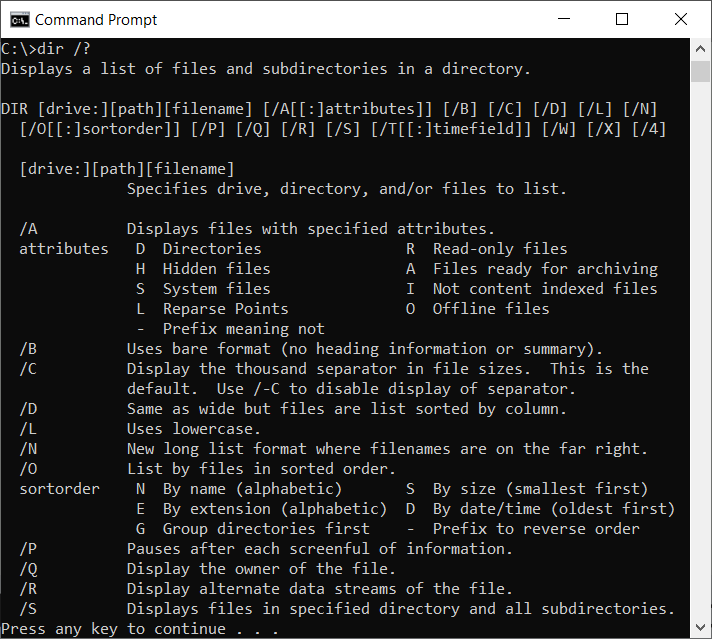
\includegraphics[width=\linewidth]{runtime-parameters-win10-cmd-dir}
	}{
		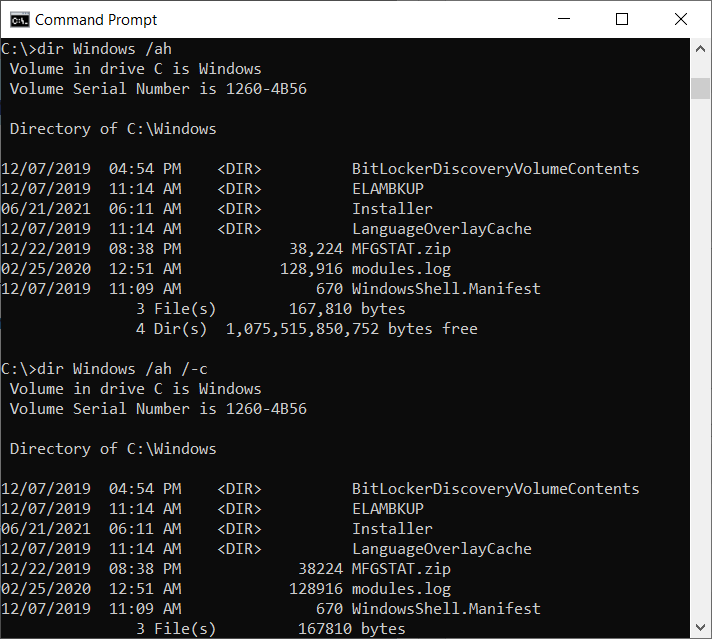
\includegraphics[width=\linewidth]{runtime-parameters-win10-cmd-dir2}
	}
\end{frame}

\subsection{Configuration Files}

\begin{frame}{Example: Configuration Files}
	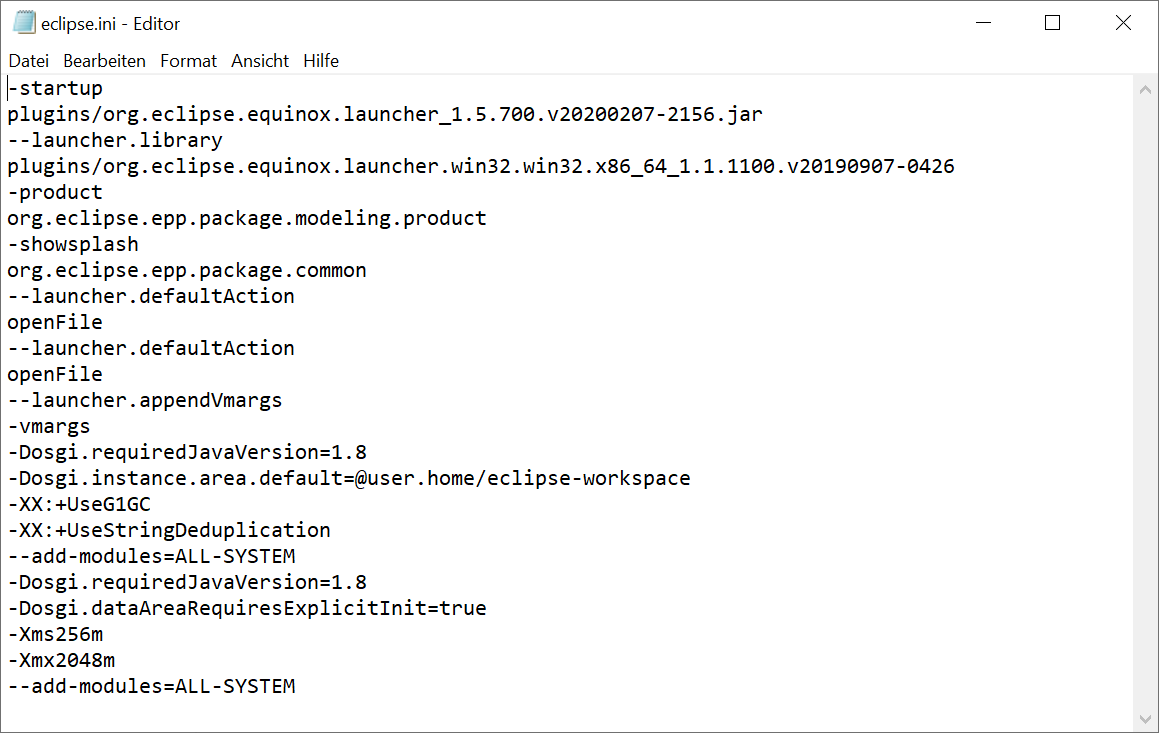
\includegraphics[width=0.75\linewidth]{configfile-eclipse-ini}
\end{frame}

\subsection{Preference Dialogs}

\begin{frame}{Example: Preference Dialogs}
	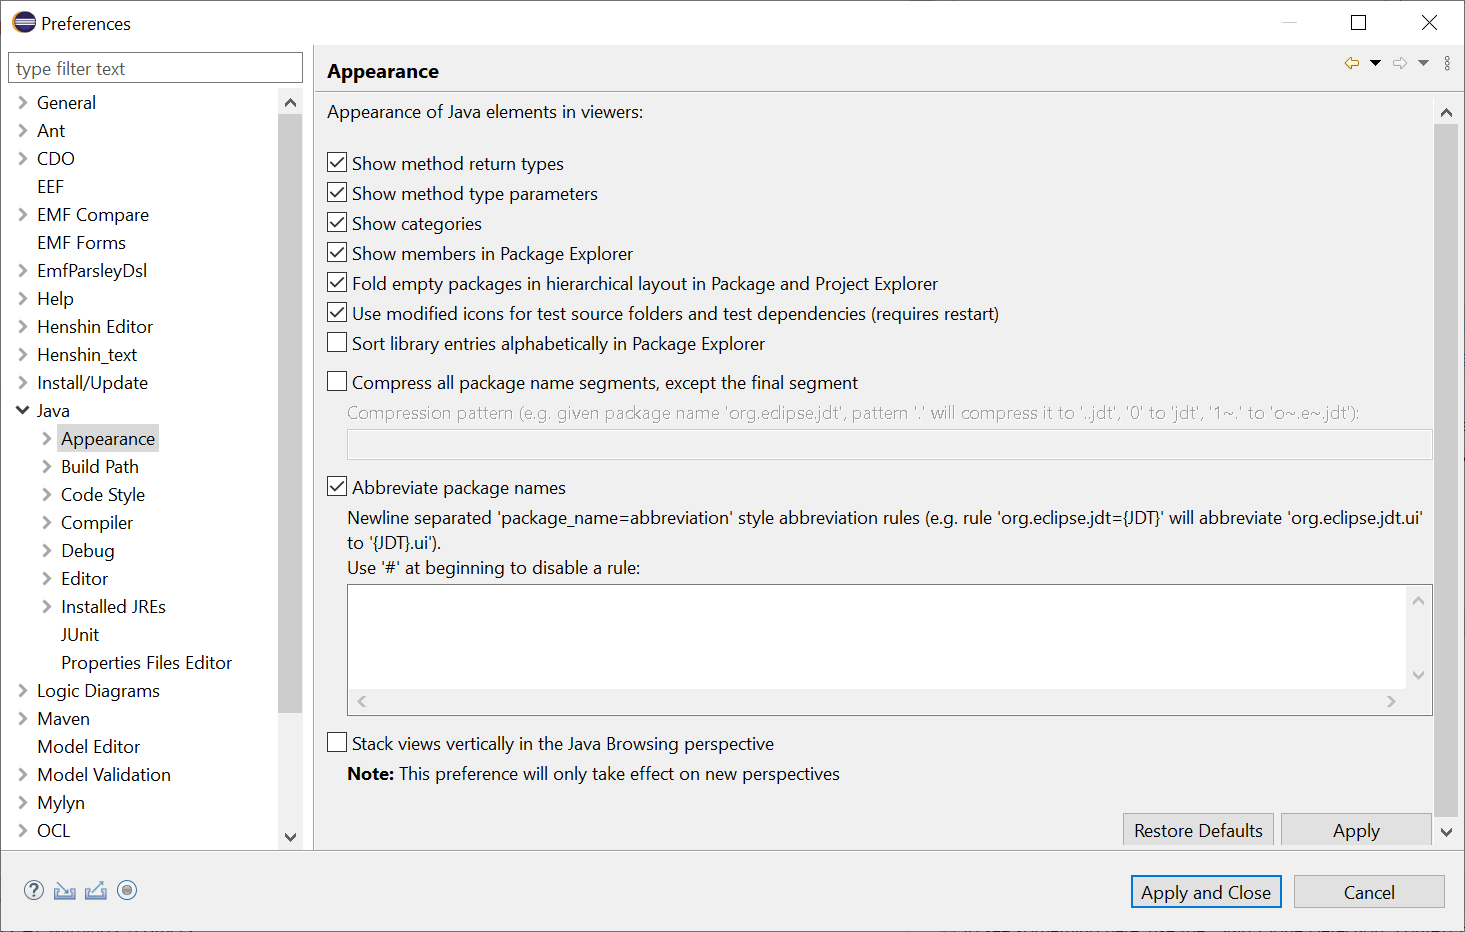
\includegraphics[width=0.75\linewidth]{preferences-eclipse}
\end{frame}

\subsection{Runtime Variability}

\begin{frame}{What do these examples have in common?}
	\begin{mycolumns}[columns=3,widths={26,36,36},animation=none]
		\pic[width=\linewidth]{runtime-parameters-win10-cmd-dir}
	\mynextcolumn
		\pic[width=\linewidth]{configfile-eclipse-ini}
	\mynextcolumn
		\pic[width=\linewidth]{preferences-eclipse}
	\end{mycolumns}
		
	\uncover<2->{
		\begin{mycolumns}[columns=2,widths={55,40},animation=none]
			\mynote{Configuration Parameters}{
				\begin{itemize}
					\item Behavior of a program is determined by configuration parameters being interpreted at runtime.
					\item In other words: Choices offered by variability are decided at runtime.
					\item Configuration may happen non-interactively (at startup) or interactively (through dialogs).
				\end{itemize}
			}			
		\mynextcolumn	
			\mydefinition{Runtime Variability\mysource{\fospl\mypage{49}}}{
				Runtime variability is decided after compilation when the program is started (aka. load-time variability) or during program execution.
			}	
		\end{mycolumns}
	}
\end{frame}

\subsection{Configuration Parameters}

\begin{frame}{Example: A Graph Library}
	A simple library providing \ldots \\
	\vspace{5mm}
	\leftorright{
		\myexample{\ldots graph data structures}{
			\begin{itemize}
				\item Directed/undirected edges
				\item Weighted/unweighted edges 
				\item Colored/uncolored nodes
				\item etc.
			\end{itemize}
		}		
	}{
		\myexample{\ldots and algorithms}{
			\begin{itemize}
				\item Vertex numbering
				\item Vertex coloring 
				\item Shortest path
				\item Minimum spanning tree 
				\item etc.
			\end{itemize}
		}
	}
\end{frame}

\begin{frame}{Features of a Graph}
	\begin{mycolumns}[columns=4,widths={25},animation=none]
		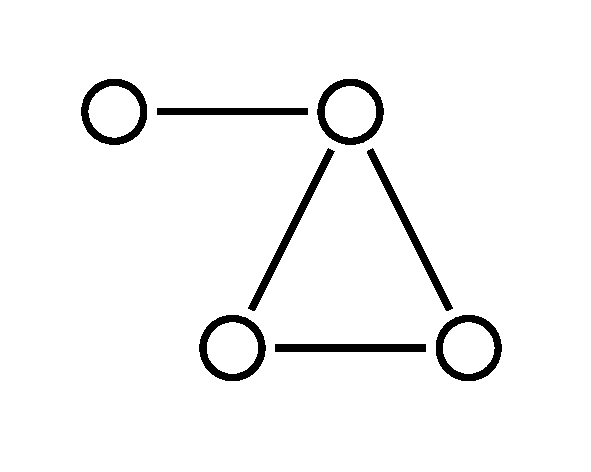
\includegraphics[width=\linewidth,page=1]{graphs}
		\includegraphics[width=\linewidth,page=3]{graphs}
		\ldots etc.
	\mynextcolumn
		\includegraphics[width=\linewidth,page=5]{graphs}
		\includegraphics[width=\linewidth,page=7]{graphs}
	\mynextcolumn
		\includegraphics[width=\linewidth,page=11]{graphs}
		\includegraphics[width=\linewidth,page=13]{graphs}
	\mynextcolumn
		\includegraphics[width=\linewidth,page=15]{graphs}
		\includegraphics[width=\linewidth,page=17]{graphs}		
	\end{mycolumns}
\end{frame}

\begin{frame}{Features as Configuration Parameters}
	\begin{mycolumns}[columns=3,widths={25,25,45},animation=none]
		\myexampletight{Directed}{\includegraphics[width=\linewidth,page=3]{graphs}}	
		\myexampletight{Colored}{\includegraphics[width=\linewidth,page=11]{graphs}}	
	\mynextcolumn
		\myexampletight{Weighted}{\includegraphics[width=\linewidth,page=5]{graphs}}	
		\myexampletight{Weighted, Colored}{\includegraphics[width=\linewidth,page=15]{graphs}}			
	\mynextcolumn
		\includegraphics[width=0.45\linewidth,page=6]{graphs}
		\hfill
		\includegraphics[width=0.45\linewidth,page=12]{graphs}
		
		~
		
		\mynote{Configuration of graph data structures}{
			\begin{itemize}
				\item Typically, configuration parameters are {\em flags}.
				\item Their boolean value determines which {\em features} are {\em activated} and which ones are {\em deactivated}.
			\end{itemize}
		}
	\end{mycolumns}
\end{frame}

\subsection{Validity of Parameter Settings}

\begin{frame}{\myframetitle}
	\begin{mycolumns}[columns=4,widths={65,5,15,15},animation=none]
		\begin{tabular}{llll}
			\toprule
			{\bf Algorithm} 							& {\bf Graph type} 	& {\bf Weights} & {\bf Coloring}  \\ \midrule
			{\em Vertex numbering}			  & *          				& *        			& *         			\\
			{\em Vertex coloring}       	& undirected 				& *        			& colored   			\\
			{\em Shortest path}        		& directed   				& weighted 			& *         			\\
			{\em Minimum spanning tree} 	& undirected 				& weighted 			& *         			\\
			\ldots         					& \ldots 			 			& \ldots 		  	& \ldots 					\\ \bottomrule
		\end{tabular}
		\vspace{5mm}	
		\uncover<2->{\mynote{Dependencies between features must be checked}{
			\begin{itemize}
				\item When the parameters are configured at startup, or
				\item whenever parameters are changed at runtime.
			\end{itemize}
		}}
	\mynextcolumn
		~
	\mynextcolumn
		\myexampletight{Directed}{\includegraphics[width=\linewidth,page=3]{graphs}}	
		\myexampletight{Colored}{
			\hfill\\
			\hfill\\
			\includegraphics[width=\linewidth,page=11]{graphs}
		}	
	\mynextcolumn
		\myexampletight{Weighted}{\includegraphics[width=\linewidth,page=5]{graphs}}	
		\myexampletight{Weighted, Colored}{\includegraphics[width=\linewidth,page=15]{graphs}}	
	\end{mycolumns}
\end{frame}
\lessonslearned{
	\item External setting of configuration options through command-line parameters, preference dialogs, configuration files
	\item Validity of combinations may be affected by dependencies between features
}{
	\item \fospl\mychapter{3}\mypages{47--49}\\--- brief introduction of binding times
	% TODO better literature pointers?
}{
	\begin{itemize}
		\item Do you know any practical examples making use of runtime variability?
		\item How does the configuration take place?
		\item Is the configuration checked for validity?
	\end{itemize}
}

\section{Realization of Runtime Variability}
\begin{frame}{Recap: Variability and Binding Times}
	\begin{mycolumns}[widths={45},animation=none]
		
\includegraphics[width=\linewidth]{metaproduct2}	
	\mynextcolumn
		\mydefinition{Binding Time}{
			\begin{itemize}
				\item Variability offers choices.
				\item Derivation of a product requires to make decisions (aka. binding).
				\item Decisions may be bound at different binding times.
			\end{itemize}
		}	
		\uncover<2->{\mynote{When, how and by whom?}{
			In the sequel: Focus on how\ldots
		}}
	\end{mycolumns}
\end{frame}

\begin{frame}[fragile]{A Non-Variable Graph Implementation}
	\begin{tiny}
		\begin{columns}
			\column{.45\textwidth}
\begin{codetight}{}
public class Graph {
	List nodes = new ArrayList();
	List edges = new ArrayList();

	Edge add(Node n, Node m) {
		Edge e = new Edge(n, m);
		nodes.add(n); nodes.add(m); edges.add(e);
		e.weight = new Weight();
		return e;
	}
	Edge add(Node n, Node m, Weight w) {
		Edge e = new Edge(n, m);
		nodes.add(n); nodes.add(m); edges.add(e);
		e.weight = w;
		return e;
	}
	void print() {
		for (int i = 0; i < edges.size(); i++) {
			((Edge) edges.get(i)).print();
		}
	}
}
\end{codetight}
\begin{codetight}{}
public class Color {
	static void setDisplayColor(Color c) {...}
}
\end{codetight}	
			\column{.45\textwidth}
\begin{codetight}{}
public class Node {
	int id = 0;
	Color color = new Color();

	void print() {
		Color.setDisplayColor(color);
		System.out.print(id);
	}
}
\end{codetight}
\begin{codetight}{}
public class Edge {
	Node a, b;
	Weight weight = new Weight();

	Edge(Node _a, Node _b) {
		a = _a; b = _b;
	}
	void print() {
		a.print(); b.print();
		weight.print();
	}
}
\end{codetight}
\begin{codetight}{}
public class Weight {
	void print() {...}
}
\end{codetight}
		\end{columns}
	\end{tiny}
\end{frame}

\begin{frame}[fragile]{``Symbolic'' Feature Traces}
	\begin{tiny}
		\begin{columns}
			\column{.45\textwidth}
\begin{codetight}{}
public class Graph {
	List nodes = new ArrayList();
	List edges = new ArrayList();

	Edge add(Node n, Node m) {
		Edge e = new Edge(n, m);
		nodes.add(n); nodes.add(m); edges.add(e);
		@e.weight = new Weight();@
		return e;
	}
	@Edge add(Node n, Node m, Weight w) {
		Edge e = new Edge(n, m);
		nodes.add(n); nodes.add(m); edges.add(e);
		e.weight = w;
		return e;
	}@
	void print() {
		for (int i = 0; i < edges.size(); i++) {
			((Edge) edges.get(i)).print();
		}
	}
}
\end{codetight}
\begin{codetight}{}
~public class Color {
	static void setDisplayColor(Color c) {...}
}~
\end{codetight}	
			\column{.45\textwidth}
\begin{codetight}{}
public class Node {
	int id = 0;
	~Color color = new Color();~

	void print() {
		~Color.setDisplayColor(color);~
		System.out.print(id);
	}
}
\end{codetight}
\begin{codetight}{}
public class Edge {
	Node a, b;
	@Weight weight = new Weight();@

	Edge(Node _a, Node _b) {
		a = _a; b = _b;
	}
	void print() {
		a.print(); b.print();
		@weight.print();@
	}
}
\end{codetight}
\begin{codetight}{}
@public class Weight {
	void print() {...}
}@
\end{codetight}
		\end{columns}
	\end{tiny}
\end{frame}

\begin{frame}[fragile]{Adding Variability: A Basic Idea}
		\begin{columns}
			\column{.45\textwidth}
				\mynote{}{
					Conditional statements, controlled by configuration parameters.
				}
				\vspace{5mm}
\begin{tiny}
\begin{codetight}{}
public class Graph {
	...
	Edge add(Node n, Node m) {
		Edge e = new Edge(n, m);
		nodes.add(n); nodes.add(m); edges.add(e);
		@if (WEIGHTED) { e.weight = new Weight(); }@
		return e;
	}
	@Edge add(Node n, Node m, Weight w) {
		if (!WEIGHTED) { throw new RuntimeException(); }
		Edge e = new Edge(n, m);
		nodes.add(n); nodes.add(m); edges.add(e);
		e.weight = w;
		return e;
	}@
	...
}
\end{codetight}
\end{tiny}	
			\column{.45\textwidth}
\begin{tiny}
\begin{codetight}{}
public class Node {
	~Color color;~
	...
	Node(){
		~if (COLORED) { color = new Color(); }~
	}
	void print() {
		~if (COLORED) { Color.setDisplayColor(color); }~
		System.out.print(id);
	}
}
\end{codetight}
\begin{codetight}{}
public class Edge {
	@Weight weight;@ 
	...
	Edge(Node _a, Node _b) {
		a = _a; b = _b;
		@if (WEIGHTED) { weight = new Weight(); }@
	}
	void print() {
		a.print(); b.print();
		@if (WEIGHTED) { weight.print(); }@
	}
}
\end{codetight}
\end{tiny}	
		\end{columns}
\end{frame}

\subsection{Global Variables}

\begin{frame}[fragile]{\myframetitle}
		\begin{columns}
			\column{.45\textwidth}
\begin{tiny}
\begin{codetight}{}
public class Config {
	~public static boolean COLORED = true;~
	@public static boolean WEIGHTED = false;@
}
\end{codetight}
\begin{codetight}{}
public class Graph {
	...
	Edge add(Node n, Node m) {
		Edge e = new Edge(n, m);
		nodes.add(n); nodes.add(m); edges.add(e);
		@if (Config.WEIGHTED) { e.weight = new Weight(); }@
		return e;
	}
	@Edge add(Node n, Node m, Weight w) {
		if (!Config.WEIGHTED) { throw new RuntimeException(); }
		Edge e = new Edge(n, m);
		nodes.add(n); nodes.add(m); edges.add(e);
		e.weight = w;
		return e;
	}@
	...
}
\end{codetight}
\end{tiny}	
			\column{.45\textwidth}
\begin{tiny}
\begin{codetight}{}
public class Node {
	~Color color;~
	...
	Node(){
		~if (Config.COLORED) { color = new Color(); }~
	}
	void print() {
		~if (Config.COLORED) { Color.setDisplayColor(color); }~
		System.out.print(id);
	}
}
\end{codetight}
\begin{codetight}{}
public class Edge {
	@Weight weight;@
	...
	Edge(Node _a, Node _b) {
		a = _a; b = _b;
		@if (Config.WEIGHTED) { weight = new Weight(); }@
	}
	void print() {
		a.print(); b.print();
		@if (Config.WEIGHTED) { weight.print(); }@
	}
}
\end{codetight}
\end{tiny}	
		\end{columns}
\end{frame}

\begin{frame}[fragile]{Special Case: Immutable Global Variables}
		\begin{columns}
			\column{.45\textwidth}
\begin{tiny}
\begin{codetight}{}
public class Config {
	~public static final boolean COLORED = true;~
	@public static final boolean WEIGHTED = false;@
}
\end{codetight}
\begin{codetight}{}
public class Graph {
	...
	Edge add(Node n, Node m) {
		Edge e = new Edge(n, m);
		nodes.add(n); nodes.add(m); edges.add(e);
		@if (Config.WEIGHTED) { e.weight = new Weight(); }@
		return e;
	}
	@Edge add(Node n, Node m, Weight w) {
		if (!Config.WEIGHTED) { throw new RuntimeException(); }
		Edge e = new Edge(n, m);
		nodes.add(n); nodes.add(m); edges.add(e);
		e.weight = w;
		return e;
	}@
	...
}
\end{codetight}
\end{tiny}	
			\column{.45\textwidth}
				\mynote{Idea}{ 
					\begin{itemize}
						\item Static configuration when configuration parameters are known at compile time.
					\end{itemize}					
				}
				\uncover<2->{\mynote{Discussion}{ 
					\begin{itemize}
						\item {\bf Advantage:} Compiler optimizations may remove dead code.
					\end{itemize}					
					\begin{itemize}
						\item {\bf Disadvantage:} No external configuration by the end-user.
					\end{itemize}
				}}
		\end{columns}
\end{frame}

\subsection{Method Parameters and Parameter Passing}
\begin{frame}[fragile]{\myframetitle}
		\begin{columns}
			\column{.45\textwidth}
\begin{tiny}
\begin{codetight}{}
public class Graph {
	@boolean weighted;@
	~boolean colored;~
	...
	Graph(@boolean _weighted@, ~boolean _colored~) {
		@weighted = _weighted;@
		~colored = _colored;~
	}
	
	Edge add(Node n, Node m) {
		Edge e = new Edge(n, m, @weighted@);
		nodes.add(n); nodes.add(m); edges.add(e);
		@if (weighted) { e.weight = new Weight(); }@
		return e;
	}
	...
}
\end{codetight}
\begin{codetight}{}
public class Edge {
	@boolean weighted;@
	@Weight weight;@ 
	...
	Edge(Node _a, Node _b, @boolean weighted@) {
		a = _a; b = _b;
		@if (weighted) { weight = new Weight(); }@
	}
	...
}
\end{codetight}
\end{tiny}	
			\column{.45\textwidth}
				\mynote{Idea}{ 
					\begin{itemize}
						\item A class exposes its configuration parameters as part of its interface (i.e., method parameters).
						\item Parameter values are passed along method invocations.
					\end{itemize}
				}				
				\uncover<2->{\mynote{Discussion}{ 
					\begin{itemize}
						\item {\bf Advantage:} Different instantiations (e.g., colored and uncolored graphs) within in the same program.
					\end{itemize}					
					\begin{itemize}
						\item {\bf Disadvantage:} May lead to methods with many parameters (code smell!).
					\end{itemize}
				}}
		\end{columns}
\end{frame}

\subsection{Reconfiguration at Runtime?}
\begin{frame}[fragile]{\myframetitle}
		\begin{columns}
			\column{.45\textwidth}
\begin{tiny}
\begin{codetight}{}
public class Config {
	~public static boolean COLORED = false;~
	@public static boolean WEIGHTED = false;@
}

\end{codetight}
\begin{codetight}{}
public class Node {
	~Color color;~
	...
	Node(){
		~if (Conf.COLORED) { 
			color = new Color(); 
		}~
	}
	void print() {
		~if (Conf.COLORED) { 
			Color.setDisplayColor(color); 
		}~
		System.out.print(id);
	}
}
\end{codetight}
\end{tiny}	
			\column{.45\textwidth}
				\mynote{Idea}{ 
					\begin{itemize}
						\item Alter feature selection without stopping and restarting the program.
					\end{itemize}
				}	
				~
				\uncover<2->{\mynote{}{
					What happens we change the value of {\tt COLORED} from {\tt false} to {\tt true} (at runtime)?
				}}
				\uncover<3->{\mynote{Discussion}{ 
					\begin{itemize} 
						\item Feature-specific code may depend on certain initialization steps or assume certain invariants.
						\item Just updating the values of configuration parameters does not update the current state of the program.
					\end{itemize}
				}}
		\end{columns}
\end{frame}

\subsection{Code Scattering}
\begin{frame}{Problem: Code Scattering}
	\begin{center}
		\vspace{-2mm}
		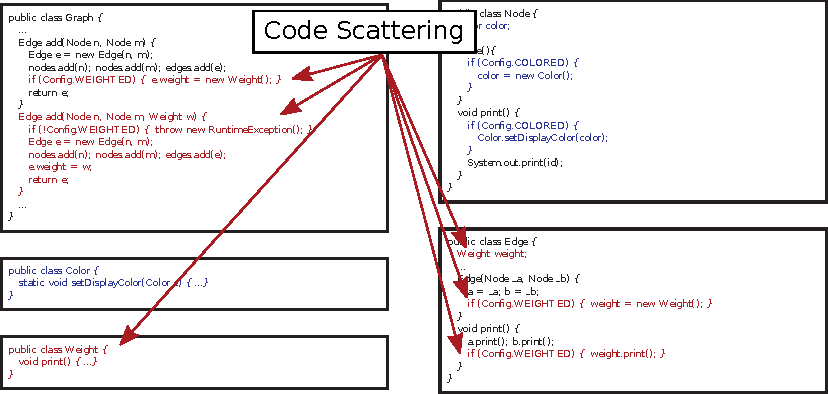
\includegraphics[scale=1.0]{scattering}
	\end{center}
\end{frame}

\subsection{Code Tangling}
\begin{frame}{Problem: Code Tangling}
	\begin{center}
		\vspace{-2mm}
		\includegraphics[scale=1.0]{tangling}
	\end{center}
\end{frame}

\subsection{Code Replication}
\begin{frame}{Problem: Code Replication}
	\begin{center}
		\vspace{-2mm}
		\includegraphics[scale=1.0]{replication}
	\end{center}
\end{frame}
\lessonslearned{
	\item Global (immutable) variables or (lengthy) parameter lists
	\item Reconfiguration at runtime is possible (in principle)
	\item Variability is spread over the entire program
	\item Variable parts are always delivered
}{
	\item \fospl\mychapter{4}
	\item \featureide\mysection{17.1}
	% TODO more details on what to expect in this literature
}{
	\begin{itemize} % die aufgaben sind ein bisschen theoretisch
		\item Why are code scattering, tangling and replication problematic?
		\item What are the problems of variable parts being always delivered?
	\end{itemize}
}

\section{Design Patterns for Variability}
% TODO several class diagrams shown here seem to be pixel graphics and should be replaced by vectorized ones

\subsection{Recap on Object-Orientation and Design Patterns}

\begin{frame}{Recap: Object Orientation}
	\begin{mycolumns}[height=50mm]
		\begin{definition}{Key Concepts}
			\begin{itemize}
				\item \textbf{Encapsulation}:\\abstraction and information hiding
				\item \textbf{Composition}:\\nested objects
				\item \textbf{Message Passing}:\\delegating responsibility
				\item \textbf{Distribution of Responsibility}:\\separation of concerns
				\item \textbf{Inheritance}:\\conceptual hierarchy, polymorphism, reuse
			\end{itemize}
		\end{definition}
	\mynextcolumn
		\picDark[width=\linewidth]{oo-concepts-illustration} % TODO what illustrates which concept? why is square not a rectangle or rectangle not a square?
	\end{mycolumns}
\end{frame}

\begin{frame}{Recap: Design Patterns\ \mytitlesource{\gof}}
	\begin{mycolumns}[widths={60}]
		\begin{definition}{Design patterns \deutsch{Entwurfsmuster}}
			\begin{itemize}
				\item Document common solutions to concrete yet frequently occurring design problems
				\item Suggest a concrete implementation for a specific object-oriented programming problem
			\end{itemize}
		\end{definition}	
		\begin{note}{Design Patterns for Variability}
			Many Gang of Four (GoF) design patterns for designing software around stable abstractions and interchangeable (i.e., variable) parts, e.g.
			\begin{itemize}
				\item Template Method
				\item Abstract Factory
				\item Decorator
			\end{itemize}
		\end{note}
	\mynextcolumn
		\picborder{\pic[width=\linewidth]{gof}}
	\end{mycolumns}
\end{frame}

\subsection{Template Method Pattern}
\begin{frame}{\myframetitle}
	\begin{mycolumns}[widths={40}]
		\begin{definition}{Template Method \mysource{\gof\mypages{325--330}}}
			\begin{itemize}
				\item {\bf Intent:} \mycite{Define the overall structure of an algorithm, while allowing subclasses to refine, or redefine, certain steps.}
				\item {\bf Motivation:}  Avoid code replication by implementing the general workflow of an algorithm once, while allowing for necessary variations.
				\item {\bf Idea:} A template method defines the skeleton of an algorithm. Concrete methods override the hook methods.
			\end{itemize}
		\end{definition}
	\mynextcolumn
		\picDark[width=\linewidth]{templatemethod}
	\end{mycolumns}
\end{frame}

\subsection{Abstract Factory Pattern}
\begin{frame}{\myframetitle}
	\begin{mycolumns}[widths={40}]
		\begin{definition}{Abstract Factory \mysource{\gof\mypages{87--95}}}
			\begin{itemize}
				\item {\bf Intent:} \mycite{Provide an interface for creating families of related or dependent objects without specifying their concrete classes.}
				\item {\bf Motivation:} Avoid case distinctions when creating objects of certain kind, consistently create objects of a particular kind.
				\item {\bf Idea:} Create classes for the consistent creation of objects.
			\end{itemize}
		\end{definition}
	\mynextcolumn
		\pic[width=\linewidth]{abstractfactory} % TODO not readible in dark mode
	\end{mycolumns}
\end{frame}

\subsection{Decorator Pattern}
\begin{frame}{\myframetitle}
	\begin{mycolumns}[widths={40}]
		\begin{definition}{Decorator \mysource{\gof\mypages{175--184}}}
			\begin{itemize}
				\item {\bf Intent:} \mycite{Attach additional responsibilities to an object dynamically. Decorators provide a flexible alternative to subclassing for extending functionality.}
				\item {\bf Motivation:} Avoid explosion of static classes when combining all additional behaviors with all applicable classes.
				\item {\bf Idea:} Create decorators and components with the same interface, whereas decorators forward behavior whenever feasible.
			\end{itemize}
		\end{definition}
	\mynextcolumn
		\picDark[width=\linewidth]{decorator}
	\end{mycolumns}
\end{frame}

\subsection{Trade-Offs and Limitations}

\begin{frame}{Object-Oriented Design of our Graph Library}
	\begin{mycolumns}[widths={40}]
		\picDark[width=\linewidth]{graphlib-oo-node-edge}
	\mynextcolumn
		\picDark[width=\linewidth]{graphlib-oo-graph}
	\end{mycolumns}
\end{frame}

\begin{frame}[fragile]{Instantiation Through Template Method Pattern}
	\small
	\begin{mycolumns}[widths={45}]
\begin{codetight}{}
class Graph {
	...
	Edge add(Node n, Node m) {
		Edge e = createEdge();
		nv.add(n); nv.add(m); ev.add(e);
		return e;
	}
	// hook method (with default implementation)
	Edge createEdge(Node n, Node m) {
		return new Edge(n, m);
	}
}
\end{codetight}
\begin{codetight}{}
@class WeightedGraph extends Graph {
	...
	// override hook method
	Edge createEdge(Node n, Node m) {
		Edge e = new WeightedEdge(n, m);
		e.weight = new Weight();
		return e;
	}
}@
\end{codetight}
	\mynextcolumn
		\centering\picDark[width=.7\linewidth]{graphlib-oo-node-edge}
	\end{mycolumns}
\end{frame}

\begin{frame}[fragile]{Instantiation Through Abstract Factory Pattern}
	\small
	\begin{mycolumns}[b]
\begin{codetight}{}
class Graph {
	EdgeFactory edgeFactory;
	...
	Graph(EdgeFactory edgeFactory) {
		this.edgeFactory = edgeFactory;
	}
	Edge add(Node n, Node m) {
		Edge e = edgeFactory.createEdge(n, m);
		nodes.add(n); nodes.add(m); edges.add(e);
		return e;
	}
}
\end{codetight}
\begin{codetight}{}
class EdgeFactory {
	Edge createEdge(Node a, Node b) {
		return new Edge(a, b);
	}
}
\end{codetight}
	\mynextcolumn
		\centering\picDark[width=.75\linewidth]{graphlib-oo-node-edge}	
\begin{codetight}{}
@class WeightedEdgeFactory extends EdgeFactory {
	Edge createEdge(Node a, Node b) {
		Edge e = new WeightedEdge(n, m);
		e.weight = new Weight();
		return e;
	}
}@
\end{codetight}
	\end{mycolumns}
\end{frame}

\begin{frame}{Feature Combinations?}
	\centering\picDark[width=.5\linewidth]{graphlib-oo-diamond}
\end{frame}

\begin{frame}{Diamond Problem}
	\begin{mycolumns}
		\begin{note}{Multiple Inheritance}
			\begin{itemize}
				\item most object-oriented programming languages do not support multiple inheritance (or only provide workarounds)
				\item critical: how to handle name clashes
			\end{itemize}
			% TODO add quote on multiple inheritance?
			% Multiple Inheritance is like a parachute. You don't often need it, but when you do, you really need it. Grady Booch? this one does not really fit here
		\end{note}
	\mynextcolumn
		\picDark[width=\linewidth]{graphlib-oo-diamond-commented}
	\end{mycolumns}
\end{frame}

\begin{frame}{Static Modeling of Feature Combinations}
	\begin{mycolumns}[columns=3,widths={10,80},animation=none]
	\mynextcolumn
		\picDark[width=\linewidth]{graphlib-oo-combinatorial}
		\mynote{}{
			Even if multiple inheritance is supported, statically combining features through inheritance is tedious (or infeasible).
		}
	\mynextcolumn
	\end{mycolumns}
\end{frame}

\begin{frame}[fragile]{Decorator Pattern as a Solution?} % TODO motivation too short
	\begin{mycolumns}[widths={52}]
		\small
\begin{codetight}{}
abstract class GraphDecorator implements IGraph {
	IGraph graph;
	GraphDecorator(IGraph graph) {
		this.graph = graph;
	}
}
\end{codetight}
\begin{codetight}{}
@class WeightedGraph extends GraphDecorator {
	WeightedGraph(IGraph graph) {
		super(graph);
	}
	Edge add(Node n, Node m) {
		WeightedEdge e = (WeightedEdge) graph.add(n, m);
		e.weight = new Weight();
		return e;
	}
	...
}@
\end{codetight} % TODO old slides had a further example. add it?
	\mynextcolumn
		\picDark[width=\linewidth]{graphlib-oo-decorator}
	\end{mycolumns}
	\small
\begin{codetight}{Example Usage}
IGraph graph = @new WeightedGraph(@~new ColoredGraph(~new Graph(@new WeightedEdgeFactory()@)~)~@)@;
\end{codetight}
\end{frame}

\begin{frame}{Delegation Instead of Inheritance}
	\begin{mycolumns}[widths={55}]
		\begin{note}{Discussion}
			Extensions (i.e., features) can be combined dynamically, but \ldots
			\begin{itemize}
				\item must be independent of each other
				\item cannot add public methods
				\item runtime overhead due to indirections
				\item several physical objects are forming a conceptual one (e.g., problems with object identity)
			\end{itemize}
		\end{note}
	\mynextcolumn
		\picDark[width=\linewidth]{graphlib-oo-decorator}
	\end{mycolumns}
\end{frame}

\lessonslearned{
	\item Variability through object-orientation and design patterns
	\item Extension through delegation vs.\ inheritance
	\item Limitations and drawbacks w.r.t.\ feature combinations
}{
	\item \oosoftwareconstruction\mychapter{3--4}
	\item \gof\mychapter{1--4}
	% TODO more details on what to expect in this literature
}{
	\begin{itemize}
		\item What characterizes a modular software design and why can it support variability?
		\item In which sense are object-oriented solutions more modular than simple conditional statements?
		\item Do you know of other design patterns supporting variability?
	\end{itemize}
}

\faq{
	\item What is variability, runtime variability, and binding time?
	\item What is the connection between variability, variability-intensive systems, and software product lines?
	\item How can configuration options be supplied?
	\item How can command-line parameters, preference dialogs, and configuration files be used to offer variability?
	\item What is the principle behind configuration options and when does the configuration happen?
	\item What are potential features of a graph library?
	\item What are examples for runtime variability? When are configuration options specified? By whom?
	\item When is the validity of configuration options checked?
}{
	\item How to realize runtime variability in source code?
	\item What is the best strategy?
	\item How can (immutable) global variables and method parameters be used to realize variability?
	%\item How to trace features in non-variable implementations?
	%\item How can configuration options be realized (for a graph library)?
	\item Why is the development of runtime variability challenging?
	\item What are code scattering, code tangling, and code replication?
	\item Does runtime variability allow reconfiguration at runtime?
	\item How to develop new features or variants with runtime variability? Exemplify!
	\item What are (dis)advantages of runtime variability?
	\item When (not) to use runtime variability?
}{
	\item What are design patterns (used for)?
	\item Why are design patterns relevant for variable software?
	\item Which design patterns are relevant for variable software?
	\item What are intent, motivation, and idea for template method, abstract factory, and decorator pattern?
	\item Given an example class diagram, which pattern is applied or should be applied? Why?
	\item What is the diamond problem? How does it affect variable software?
	\item Is multiple inheritance useful to combine features? Exemplify!
	\item What are limitations of design patterns (for variable software)?
}

\mode<beamer>{
	\begin{frame}{\inserttitle}
		\lectureseriesoverview
	\end{frame}

	\contentoverview
}


% TODO L03 COMPILE-TIME VARIABILITY WITH CLONE-AND-OWN

\ifuniversity{recording}{\date{April 22, 2023}\setpicture[200]{apr21-south}\setcopyright{}}
\ifuniversity{ulm}{\date{April 27, 2023}\setpicture[200]{apr21-south}}
\ifuniversity{magdeburg}{\setpicture[70]{ovgu-autumn2}\setcopyright{Photo: Hannah Theile (OVGU)}}

\author{Timo Kehrer, Thomas Thüm, Elias Kuiter}
\lecture{Compile-Time Variability with Clone-and-Own}{cloneandown}

\section{Compile-Time Variability and Clone-and-Own}
\subsection{Recap: Runtime Variability}
\begin{frame}{\insertsubsection}
	\leftorright{
		Basic principles
		\mynote{Runtime parameters}{
			\begin{itemize}
				\item Conditional statements controlled by configuration parameters
				\item Global variables vs. method parameter passing
			\end{itemize}	
		}
		\mynote{Object-oriented concepts and Design Patterns}{
			\begin{itemize}
				\item Template Method
				\item Abstract Factory
				\item Decorator
				\item etc.
			\end{itemize}	
		}
	}{
Problems

Configuration parameters:
Code scattering, tangling, and replication.
	
Design patterns
Trade-offs and potential negative side effects.
Constraints that may restrict their usage.
	
More generally: 
Not well-suited for compile-time binding. 
Variable parts are always delivered.
	}
\end{frame}

\begin{frame}[fragile]{A Basic Graph Implementation}
	\vspace{-1.5cm}
	\begin{flushright}
		\includegraphics[scale=0.5]{graph-basic}
	\end{flushright}
	\vspace{0.1cm}
	\begin{tiny}
		\begin{columns}
			\column{.45\textwidth}
\begin{lstlisting}
public class Graph {
	List nodes = new ArrayList();
	List edges = new ArrayList();

	Edge add(Node n, Node m) {
		Edge e = new Edge(n, m);
		nodes.add(n); nodes.add(m); edges.add(e);
		return e;
	}
	void print() {
		for (int i = 0; i < edges.size(); i++) {
			((Edge) edges.get(i)).print();
		}
	}
}
\end{lstlisting}
			\column{.45\textwidth}
\begin{lstlisting}
public class Node {
	int id = 0;

	void print() {
		System.out.print(id);
	}
}
\end{lstlisting}
\begin{lstlisting}
public class Edge {
	Node a, b;

	Edge(Node _a, Node _b) {
		a = _a; b = _b;
	}
	void print() {
		a.print(); b.print();
	}
}
\end{lstlisting}
		\end{columns}
	\end{tiny}
\end{frame}

\begin{frame}[fragile]{Evolution Step: Weighted Graphs}
	\vspace{-1.5cm}
	\begin{flushright}
		\includegraphics[scale=0.5]{graph-basic-to-weighted}
	\end{flushright}
	\vspace{0.1cm}
	\begin{tiny}
		\begin{columns}
			\column{.45\textwidth}
\begin{lstlisting}
public class Graph {
	List nodes = new ArrayList();
	List edges = new ArrayList();

	Edge add(Node n, Node m) {
		Edge e = new Edge(n, m);
		nodes.add(n); nodes.add(m); edges.add(e);
		@e.weight = new Weight();@
		return e;
	}
	@Edge add(Node n, Node m, Weight w) {
		Edge e = new Edge(n, m);
		nodes.add(n); nodes.add(m); edges.add(e);
		e.weight = w;
		return e;
	}@
	void print() {
		for (int i = 0; i < edges.size(); i++) {
			((Edge) edges.get(i)).print();
		}
	}
}
\end{lstlisting}
			\column{.45\textwidth}
\begin{lstlisting}
public class Edge {
	Node a, b;
	@Weight weight = new Weight();@

	Edge(Node _a, Node _b) {
		a = _a; b = _b;
	}
	void print() {
		a.print(); b.print();
		@weight.print();@
	}
}
\end{lstlisting}
\begin{lstlisting}
@public class Weight {
	void print() {...}
}@
\end{lstlisting}
		\end{columns}
	\end{tiny}
\end{frame}

\begin{frame}[fragile]{Evolution Step: Colored Graphs}
	\vspace{-1.5cm}
	\begin{flushright}
		\includegraphics[scale=0.5]{graph-basic-to-colored}
	\end{flushright}
	\vspace{0.1cm}
	\begin{tiny}
		\begin{columns}
			\column{.45\textwidth}
\begin{lstlisting}
public class Graph {
	List nodes = new ArrayList();
	List edges = new ArrayList();

	Edge add(Node n, Node m) {
		Edge e = new Edge(n, m);
		nodes.add(n); nodes.add(m); edges.add(e);
		return e;
	}
	void print() {
		for (int i = 0; i < edges.size(); i++) {
			((Edge) edges.get(i)).print();
		}
	}
}
\end{lstlisting}	
			\column{.45\textwidth}
\begin{lstlisting}
public class Node {
	int id = 0;
	~Color color = new Color();~

	void print() {
		~Color.setDisplayColor(color);~
		System.out.print(id);
	}
}
\end{lstlisting}
\begin{lstlisting}
~public class Color {
	static void setDisplayColor(Color c) {...}
}~
\end{lstlisting}
		\end{columns}
	\end{tiny}
\end{frame}

\begin{frame}{Problem: Dealing With New Requirements}
	\leftorright{
		\myexample{New requirement}{
			\includegraphics[scale=0.4]{graph-weighted-colored}
		}
	}{
		\myexample{Where to start from?}{
			\includegraphics[scale=0.4]{graph-basic}
			\includegraphics[scale=0.4]{graph-weighted}
			\includegraphics[scale=0.4]{graph-colored}
		}
	}
\end{frame}

\begin{frame}[fragile]{Problem: Evolution and Maintenance}
	\begin{columns}
		\column{.15\textwidth}
			\includegraphics[width=\linewidth]{graph-weighted}
		\column{.3\textwidth}
\begin{tiny}
\begin{lstlisting}
public class Graph {
	...
	Edge add(Node n, Node m) {
		Edge e = new Edge(n, m);
		nodes.add(n); nodes.add(m); edges.add(e);
		@e.weight = new Weight();@
		return e;
	}
	@Edge add(Node n, Node m, Weight w) {
		Edge e = new Edge(n, m);
		nodes.add(n); nodes.add(m); edges.add(e);
		e.weight = w;
		return e;
	}@
	...
}
\end{lstlisting}
\end{tiny}
		\column{.025\textwidth}
			\begin{LARGE}
				$\Rightarrow$
			\end{LARGE}
		\column{.3\textwidth}
\begin{tiny}
\begin{lstlisting}
public class Graph {
	...
	Edge add(Node n, Node m) {
		Edge e = new Edge(n, m);
		nodes.add(n); nodes.add(m); edges.add(e);
		@e.weight = new Weight();@
		return e;
	}
	@Edge add(Node n, Node m, Weight w) {
		Edge e = this(n, m);
		e.weight = w;
		return e;
	}@
	...
}
\end{lstlisting}
\end{tiny}
	\end{columns}
	\myexample{Where and how to propagate the improvement (here: refactoring)}{
		\includegraphics[scale=0.4]{graph-basic}
		\includegraphics[scale=0.4]{graph-colored}
		\includegraphics[scale=0.4]{graph-weighted-colored}
	}
\end{frame}
\lessonslearned{
	\item Compile-time variability is decided before or at compile time
	\item In clone-and-own, new variants of a software system are created by copying and adapting an existing variant
	\item Simple paradigm, but suffering from maintenance problems in the long run
}{
	\item\fospl\mysection{3.1.1}\mypages{48--49}\\--- brief introduction of compile-time variability
	\item\softwareclonedetection\mysection{2}\mypages{1167--1168}\\--- brief introduction to software clones, their types, reasons, (dis)advantages
	\item\virtualplatform\ --- brief introduction to ad-hoc clone-and-own (L0)
	% TODO better literature pointers on clone-and-own?
}{
	\begin{itemize}
		\item What are the reasons why clone-and-own is very popular in practice?
		\item What is the order of magnitude of the number of variants that can be reasonably maintained in clone-and-own?
		\item Have you ever applied the principle of clone-and-own? If so, where and how?
	\end{itemize}
}

\section{Clone-and-Own with Version Control}

\subsection{Software Configuration Management}

\begin{frame}{Excursus: Software Configuration Management}
	\frameSoftwareConfigurationManagement
\end{frame}

\begin{frame}{Excursus: Software Configuration Management}
	\begin{mycolumns}[widths={45},animation=none]
		\begin{definition}{Basic Terms and Definitions} % TODO source missing
			\begin{itemize}
				\item {\bf Software Item}: An (atomic) artifact that can be uniquely identified
				\item {\bf Version}: A modified software item
				\begin{itemize}
					\item {\bf Revision}: A new version that replaces an old one
					\item {\bf Variant}: A version that co-exists with another one
				\end{itemize}
				\uncover<2->{
					\item {\bf Configuration}: A set of software items that together form a functioning (partial) system % TODO term is confusing and overloaded in next lecture + it appears to me that this was only needed in the good old days with CVS with versioning on a per file basis
					\item {\bf Baseline}: A stable configuration that represents a point of reference for further development
					\item {\bf Release}: A baseline delivered to customers
				}
			\end{itemize}
		\end{definition}
	\mynextcolumn
		\only<1|handout:0>{\pic[width=\linewidth]{configuration-management-1}}%
		\only<2-|handout:1>{\pic[width=\linewidth]{configuration-management-2}}%
	\end{mycolumns}	
\end{frame}

\begin{frame}{Example: A Conceptual Organization of our Graph Library}
	\centering
	\only<1|handout:0>{\pic[width=0.8\linewidth]{configuration-management-graphs-1}}%
	\only<2-|handout:1>{\pic[width=0.8\linewidth]{configuration-management-graphs-2}}%
\end{frame}
% TODO axis labels missing on this slide

%\begin{frame}{Tool Support: Version Control Systems}
	%\only<1|handout:0>{\pic[width=\linewidth,page=1]{branching}}%
	%\only<2|handout:0>{\pic[width=\linewidth,page=2]{branching}}%
	%\only<3-|handout:1>{\pic[width=\linewidth,page=3]{branching}}%
%\end{frame}

\subsection{Version Control Systems}

\begin{frame}{Tool Support: Version Control Systems}
	\centering
	\uncover<4->{\hspace{30mm}$\text{cherrypick := patch}(\Delta(r8,r10),r11)$}

	\vfill
	\only<1|handout:0>{\pic[width=0.6\linewidth]{versioncontrol-1}}%
	\only<2|handout:0>{\pic[width=0.6\linewidth]{versioncontrol-2}}%
	\only<3-|handout:1>{\pic[width=0.6\linewidth]{versioncontrol-3}}\\

	\vfill
	\uncover<5->{$\text{merge := 3-way-merge}(r4,\Delta(r4,r7),\Delta(r4,r9))$}
\end{frame}
% TODO no actual merges shown, only fast-forward
% TODO cherry pick needs to point to an arrow, not a node

\subsection{Supporting Clone-and-Own Development}

\begin{frame}{Example: Graph Library under Version Control}
	\centering\pic[width=0.7\linewidth]{versioncontrol-graphs-1}
\end{frame}

\begin{frame}{Example: Graph Library under Version Control}
	\centering\pic[width=0.7\linewidth]{versioncontrol-graphs-2}
\end{frame}

\begin{frame}{Example: Graph Library under Version Control}
	\centering\pic[width=0.7\linewidth]{versioncontrol-graphs-3}
\end{frame}

\subsection{Discussion}

\begin{frame}{Clone-and-Own with Version Control}
	\begin{mycolumns}[widths={60}]
		\begin{note}{Observations}
			\begin{itemize}
				\item aka.\ \emph{managed clone-and-own} (opposed to ad-hoc clone-and-own)
				\item Supports keeping tracking of revisions and variants\\-- aka.\ \emph{provenance} \deutsch{Herkunft}
				\item Creation of new variants is partially supported by merging of branches
				\item Propagation of changes between variants is supported by cherrypicking changes
			\end{itemize}
			However:
			\begin{itemize}
				\item Versioning is typically limited to entire system variants (i.e., branches)
				\item No flexible combination of software items
			\end{itemize}
		\end{note}
	\mynextcolumn
		\begin{note}{Advantages}
			\begin{itemize}
				\item Well-established and stable systems
				\item Well-known known process
				\item Good tool integration	
			\end{itemize}
		\end{note}
		\begin{note}{Disadvantages}
			\begin{itemize}
				\item Development of variants, not features: flexible combination of features not directly possible
				\item No structured reuse (copy \& edit)
				\item Merging and cherrypicking not fully automated
			\end{itemize}	
		\end{note}
	\end{mycolumns}
\end{frame}

\lessonslearned{
	\item Software configuration management as a traditional discipline of managing the evolution of variability-intensive systems
	\item Version control systems as a widespread tool supporting clone-and-own in practice
}{
	\item \fospl\mysection{5.1}\mypages{99--105}\\--- introduction of variability with version control (not~explicitly calling it clone-and-own)
	\item \staplesandhill\ --- experience report on managed clone-and-own with version control and build systems
	\item\virtualplatform\ --- brief introduction to clone-and-own with version control (L1)
	% TODO add literature? \summerville\mychapter{25}
}{
	\begin{itemize}
		\item Which software configuration management concepts are supported by version control systems? % TODO rather abstract question
		\item Do you know other version control systems than Git?  % TODO my feeling was that most students do not know anything beyond git and it does hot help to discuss this in groups
		\item If so, in which way are they different from Git?
		% TODO what about asking about differences between forks and branches? and what would be different with forks? when do they prefer forks/branches?
	\end{itemize}
}

\section{Clone-and-Own with Build Systems}

\begin{frame}{Recap: Software Configuration Management}
	\vspace{2mm}
	\pic[width=0.7\linewidth]{configuration-management-2}
\end{frame}

\subsection{Build Systems}

\begin{frame}{Tool Support: Build Systems}
	\begin{mycolumns}[columns=2,widths={50,50},animation=none]
		\pic[width=\linewidth]{ant-hello-world}		
	\mynextcolumn
		\mydefinition{Build Systems}{	
			\begin{itemize}
				\item Automation of the build process through build scripts
				\item Multiple steps with dependencies/conditions
				\begin{itemize}
					\item Copy files, 
					\item call compiler, 
					\item start other tools, 
					\item \ldots
				\end{itemize}	
				\item Tools: 
				\begin{itemize}
					\item make
					\item ant
					\item maven
					\ldots
				\end{itemize}
			\end{itemize}
		}
	\end{mycolumns}	
\end{frame}

\subsection{Variability through Build Scripts}

\begin{frame}{Variability through Build Scripts}
	\begin{flushright}		
		\vspace{-1cm}
		\pic[scale=0.27]{buildsystems}
		~~~~~~~~~~~~~~~~~
	\end{flushright}
	\begin{mycolumns}[columns=2,widths={50,50},animation=none]
		\vspace{-8cm}
		\mynote{Basic Idea}{	
			\begin{itemize}
				\item One build script per variant.
				\item Include/exclude files when translating.
				\item Overwrite variant-specific files.
			\end{itemize}
		}		
	\mynextcolumn
		~	
	\end{mycolumns}	
\end{frame}

\begin{frame}[fragile]{Example: Graph Library}
\begin{tiny}	
	\begin{mycolumns}[columns=4,widths={10,30,10,60},animation=none]
		~
	\mynextcolumn
		\vspace{2mm}
		\pic[width=\linewidth]{buildsystems-graphs-1}	% ist die fehlende Kante zu Graph beabsichtigt? das kann ja nicht klappen, oder?
	\mynextcolumn
		~
	\mynextcolumn
\begin{codetight}{}
public class Edge {
	Node a, b;

	Edge(Node _a, Node _b) {
		a = _a; b = _b;
	}
	...
}
\end{codetight}
\vspace{1cm}
\begin{codetight}{}
public class Edge {
	Node a, b;
	@Weight weight = new Weight();@

	Edge(Node _a, Node _b) {
		a = _a; b = _b;
	}
	...
}
\end{codetight}
	\end{mycolumns}
\end{tiny}
\end{frame}

\begin{frame}[fragile]{Example: Graph Library}
\begin{tiny}	
	\begin{mycolumns}[columns=4,widths={10,30,10,60},animation=none]
		~
	\mynextcolumn
		\vspace{2mm}
		\pic[width=\linewidth]{buildsystems-graphs-2}	
	\mynextcolumn
		~
	\mynextcolumn
\begin{codetight}{}
public class Graph implements IGraph {
	@EdgeFactory ef;@
	...
	@public Graph(EdgeFactory _ef) {
		ef = _ef;@
	}
	public Edge add(Node n, Node m) {
		@Edge e = ef.createEdge(n, m);@
		nodes.add(n); nodes.add(m); edges.add(e);
		return e;
	}
	...
}
\end{codetight}
\begin{codetight}{}
public class Edge {
	Node a, b;
	...
}
\end{codetight}
\vspace{0.5cm}
\begin{codetight}{}
public class WeightedEdge extends Edge {
	Node a, b;
	@Weight weight = new Weight();@
	...
}
\end{codetight}
	\end{mycolumns}
\end{tiny}
\end{frame}

\subsection{Discussion}

\begin{frame}{Discussion}
	\begin{flushright}		
		\vspace{-1cm}
		\pic[scale=0.27]{buildsystems}
		~~~~~~~~~~~~~~~~~
	\end{flushright}
	\begin{mycolumns}[columns=2,widths={50,50},animation=none]
		\vspace{-8cm}
		\mynote{Comparison to Version Control Systems}{	
			\begin{itemize}
				\item Supports combination of more fine-grained software items (i.e., files).
				\item However: No provenance support.
			\end{itemize}
		}	
		\mynote{More generally:}{	
			\begin{itemize}
				\item Combination of items (i.e., files) $\neq$ combination of features.
				\item All variants are potentially affected by changes to the basic variant.
			\end{itemize}
		}		
	\mynextcolumn
		~	
	\end{mycolumns}	
\end{frame}
\lessonslearned{
	\item Variability through build scripts
	\item Granularity of clones: Individual files
	\item Combination of files\\$\neq$ combination of features
}{
	\item \fospl\mysection{5.2.2 and 5.2.4}\mypages{106--110}\\--- brief introduction of clone-and-own with build systems (not~explicitly calling it clone-and-own)
	\item \staplesandhill\ --- experience report on managed clone-and-own with version control and build systems
}{
	\begin{itemize}
		\item Which software configuration management concepts are supported by build systems?
		\item What are the commonalities and differences of clone-and-own with version control and clone-and-own with build systems?
		\item What are the strengths and weaknesses?
		% TODO \item What is the effort to convert ad-hoc clone-and-own into managed clone-and-own?
	\end{itemize}
}

\faq{
	\item What are problems of runtime variability?
	\item What is compile-time variability?
	\item What is (ad-hoc) clone-and-own?
	\item How to develop new features or variants? Exemplify!
	\item What are (dis)advantages of (ad-hoc) clone-and-own?
	\item When (not) to use (ad-hoc) clone-and-own?
	\item What is better runtime or compile-time variability?
}{
	\item What is software configuration management and version control (used~for)?
	\item What is the difference between version, revision, variant, configuration, baseline, release, merge, cherrypick, revision control?
	\item How can version control be used for clone-and-own? Illustrate!
	\item How to develop new features or variants? Exemplify!
	\item What are (dis)advantages of version control for variability?
	\item When (not) to use clone-and-own with version control?
	\item Shall we use version control at all?
}{
	\item What are build systems (used~for)?
	\item How can build systems be used for clone-and-own? Illustrate!
	\item How to develop new features or variants? Exemplify!
	\item What are (dis)advantages of build systems for variability?
	\item When (not) to use clone-and-own with build systems?
	\item Shall we use build systems at all?
	\item What is the granularity of clones for all three techniques?
	\item What is the effort to migrate from ad-hoc clone-and-own to managed clone-and-own?
}

\mode<beamer>{
	\begin{frame}{\inserttitle}
		\lectureseriesoverview
	\end{frame}

	\contentoverview
}

